% Requires in preamble:
% \usepackage{tikz}
% \usetikzlibrary{decorations.pathreplacing}
\subsubsection{Youtube proof example}

% ---------------------------------------------------------
% Toolkit
% ---------------------------------------------------------
\begin{tcolorbox}[title=Toolkit: Youtube Proof]
\begin{tabular}{@{}p{0.28\textwidth}p{0.68\textwidth}@{}}
\textbf{Core items} & Key definitions/results introduced in this file.\\
\textbf{How to use} & Read the boxed items first; proofs and consequences follow.\\
\textbf{Dependencies} & Refer back to earlier sections as needed.\\
\end{tabular}
\end{tcolorbox}

\begin{proof}
Let $\{a_n\}$ be a monotone increasing sequence that is bounded above.

Let
\[
E := \{ a_n \mid n \in \mathbb{N} \}.
\]
Then $E \neq \varnothing$ and $E$ is bounded above.

Let
\[
a := \sup E.
\]
We will show that
\[
\lim_{n \to \infty} a_n = a.
\]

Let $\varepsilon > 0$ be given.

By definition of supremum, $a - \varepsilon$ is not an upper bound for $E$.
Hence,
\[
\exists\, n_0 \in \mathbb{N}
\quad \text{such that} \quad
a - \varepsilon < a_{n_0} \le a.
\]

Because $\{a_n\}$ is monotone increasing,
\[
a - \varepsilon < a_n \le a
\quad \text{for all } n \ge n_0.
\]

\begin{center}
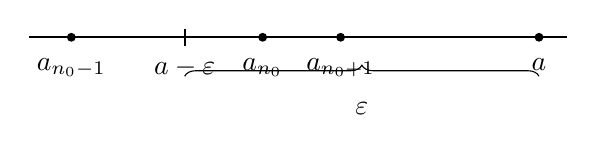
\begin{tikzpicture}[x=0.9cm,y=0.9cm,>=stealth]
  % --- choose positions (kept compact for letter paper) ---
  \def\xLeft{0}
  \def\xAe{2.2}
  \def\xAnz{3.3}
  \def\xAnzp{4.4}
  \def\xA{7.2}

  % number line
  \draw[thick] (\xLeft,0) -- (\xA+0.4,0);

  % tick at a-ε
  \draw[thick] (\xAe,0.12) -- (\xAe,-0.12);

  % points
  \fill (\xLeft+0.6,0) circle (1.6pt) node[below=4pt] {$a_{n_0-1}$};
  \fill (\xAnz,0)      circle (1.6pt) node[below=4pt] {$a_{n_0}$};
  \fill (\xAnzp,0)     circle (1.6pt) node[below=4pt] {$a_{n_0+1}$};
  \fill (\xA,0)        circle (1.6pt) node[below=4pt] {$a$};

  % label a-ε under tick
  \node[below=4pt] at (\xAe,0) {$a-\varepsilon$};

  % epsilon brace from a-ε to a
  \draw[decorate,decoration={brace,amplitude=4pt}]
    (\xAe,-0.55) -- (\xA,-0.55)
    node[midway,below=6pt] {$\varepsilon$};

  % optional: subtle note above (kept short)
  % \node[above=6pt] at ({(\xAe+\xA)/2},0) {$a-\varepsilon < a_n \le a$ for $n\ge n_0$};
\end{tikzpicture}
\end{center}

Thus,
\[
a_n \in N_\varepsilon(a)
\quad \text{for all } n \ge n_0.
\]
This is precisely the definition of convergence. Therefore,
\[
\lim_{n \to \infty} a_n = a.
\]
\end{proof}
